\chapter*{Conclusion and outlook}\label{chap:Conclusions}
\chaptermark{Conclusion and outlook}
\markboth{\MakeUppercase{Conclusion and outlook}}{}
\addcontentsline{toc}{chapter}{Conclusion and outlook}

\renewcommand\thefigure{C\arabic{figure}} 
\setcounter{figure}{0}

In this thesis, we elucidated two classes of the commonly encountered free-surface phenomena: the impact of liquid drops on non-wetting substrates (part~\ref{PartA}), and capillary-driven retraction and bursting of films and free-surface bubbles (part~\ref{PartB}). Figure~\ref{Fig::Conclusion} summarizes the different regimes observed in this thesis. We also show the range of dimensionless numbers simulated to explore these regimes. In this section, we will briefly revisit each chapter to summarize the key results and answer the questions posed in the introduction to this thesis. We also point out open issues and propose follow-up studies that may stem from the various chapters.

\begin{sidewaysfigure}
	\centering
	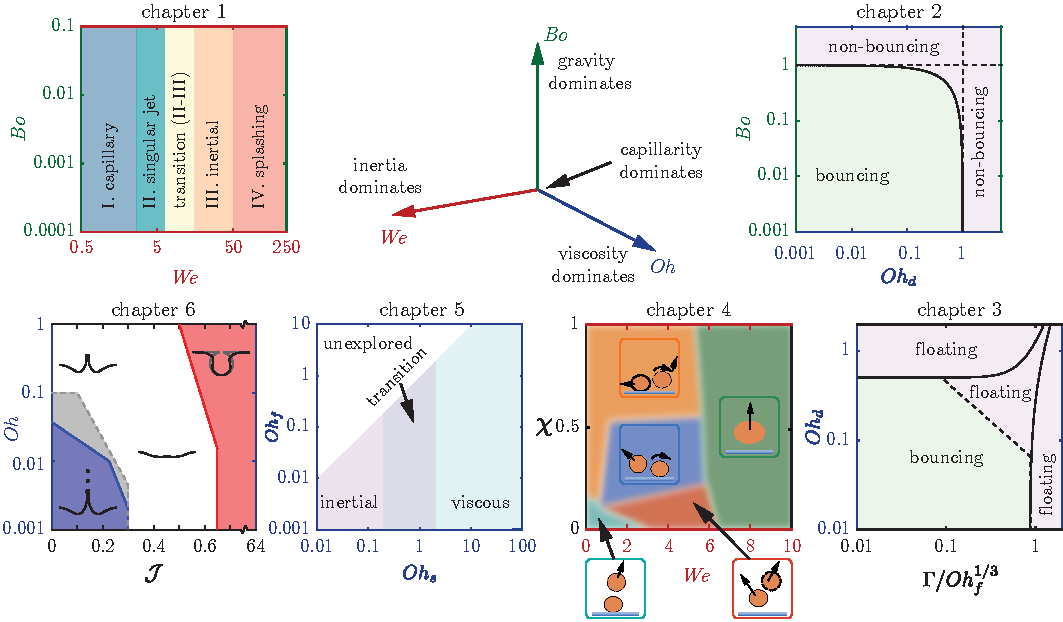
\includegraphics[width=180mm]{FiguresMisc/ConclusionRegimes_v4.pdf}	
	\caption{Summary of the different regimes and the range of the dimensionless numbers simulated to explore these regimes. The different regime maps contain the Weber number $\Wen$ (equation~\eqref{Ch0::We}, chapters~\ref{chap:DropForces} and~\ref{chap:DropOnDrop}), the Bond number $\Bon$ (equation~\eqref{Ch0::Bo}, chapters~\ref{chap:DropForces} and~\ref{chap:DropViscousBouncing}), dimensionless film thickness $\Gamma$ (equation~\eqref{Ch0::Gamma}, chapter~\ref{chap:DropBouncingOnFilm}), the dimensionless offset $\chi$ (equation~\eqref{Ch0::X}) between the impacting and sessile drops (chapter~\ref{chap:DropOnDrop}), and the plasto-capillary number $\mathcal{J}$ (equation~\eqref{Ch0::J}, chapter~\ref{chap:BurstingBubbleVP}). A common theme among most of these regime maps is the use of Ohnesorge numbers $\Ohn$ (equation~\eqref{Ch0::Oh}) which can be further classified as: the drop Ohnesorge number (chapters~\ref{chap:DropViscousBouncing} and~\ref{chap:DropBouncingOnFilm}), the film Ohnesorge number $\Ohf$ (chapters~\ref{chap:DropBouncingOnFilm} and~\ref{chap:TaylorCulick}), and the surroundings Ohnesorge number $\Ohs$ (chapter~\ref{chap:TaylorCulick}). Please refer to the individual chapters for the details of each regime map.}
	\label{Fig::Conclusion}
\end{sidewaysfigure}

\section*{Part~\ref{PartA}}

In \textbf{chapter~\ref{chap:DropForces}}, we study water drops impacting non-wetting substrates and find that not only is the inertial shock at impact associated with a distinct peak in the temporal evolution of the normal force, but so is the jump-off, which was hitherto unknown. We also give the following takeaway messages:\vspace{2mm}

\todoChOne{inline,caption={},inlinewidth=\textwidth}{
	\underline{Takeaway messages \textbf{Chapter~\ref{chap:DropForces}}}
	\begin{enumerate}
		\item For most cases, the inertial pressure force sets the magnitude of both the peaks in the normal reaction force. But, surprisingly, even low-velocity impacts can lead to a remarkably high second peak in the normal force, which can even be larger than the first one.
		\item The first peak occurs immediately after impact at a time instant that conforms to the inertial shock of impact, whereas the time at which the second peak occurs scales with the inertio-capillary time owing to the drop impact and drop oscillation analogy.  
\end{enumerate}}\vspace{2mm}

The amplitude of the second peak further divides the drop impact dynamics into four distinct regimes based on the Weber number $\Wen$, I. capillary, II. singular, III. inertial, and IV. splashing. These regimes are independent of the Bond number $\Bon$ (figure~\ref{Fig::Conclusion}) for $0 < \Bon < 0.1$. In the inertial limit (low Ohnesorge numbers $\Ohn$), gravity only dictates the dynamics of the falling drop prior to its impact on the substrate. This effect is accounted in the impact velocity and hence $\Wen$. The insights from this chapter are crucial to develop countermeasures to the failure of superhydrophobicity in technological applications. Exciting and relevant extensions of our work include the study of impact forces of viscous drops, which will show quite different scaling behavior \cite{jha2020viscous}, and of Leidenfrost drops \cite{quere2013leidenfrost}. It will also be interesting to extend this work to less superhydrophobic substrates where contact line motion (viscous stresses vs. capillary traction) may significantly affect the flow focusing and hence the theoretical model. For such cases, we speculate the absolute numbers might change; however, the scaling relations would be the same.\\

In \textbf{chapter~\ref{chap:DropViscousBouncing}}, we observed that close to the bouncing to non--bouncing transition of drops falling on a non-wetting substrate, the rebound process is independent of the impact parameters. This observation disentangles the later stages of the rebound from the initial impact dynamics. Consequently, we draw an analogy to the case of coalescence-induced jumping of two identical drops \citep{boreyko2009, mouterde2017merging, lecointre2019ballistics} to give a simple criterion for the bouncing to non--bouncing transition, namely that the sum of the drop Ohnesorge and Bond numbers is unity ($\Ohn + \Bon = 1$), for the bouncing to non--bouncing transition (figure~\ref{Fig::Conclusion}). We further provide the following takeaway messages:\vspace{2mm}

\todoChTwo{inline,caption={},inlinewidth=\textwidth}{
	\underline{Takeaway messages \textbf{Chapter~\ref{chap:DropViscousBouncing}}}
	\begin{enumerate}
		\item Throughout the drop impact process, viscous dissipation enervates internal momentum. A drop will cease bouncing and stay on the substrate if its upward momentum (driven by capillarity and resisted by viscous stresses) after the retraction stage is insufficient to overcome gravity.
		\item Drops smaller than their visco-capillary length stop bouncing due to viscous dissipation \citep{jha2020viscous}.
		\item On the other hand, drops larger than their gravito-capillary length cannot bounce due to their own weight \citep{biance2006}.
\end{enumerate}}\vspace{2mm}

We stress that this chapter only deciphers the theoretical upper bound of the bouncing to non-bouncing transition on an ideal non-wetting substrate. A natural extension of this work would be to non-ideal superhydrophobic substrates and understand why the transition to non-bouncing occurs way below \citep{sarma2022interfacial} the threshold proposed in this chapter. Furthermore, we solely focus on drops impacting with velocities exceeding their inertio-capillary velocity, ie., the impact Weber numbers greater than unity. It will be interesting to extend this work for cases where the drops only deform weakly, i.e., capillarity dominates over inertia. One can either use a quasi-static model of bouncing drops \citep{molavcek2012quasi} or an analogy to non-linear springs \citep{chevy2012liquid} to probe that regime. Lastly, it will be interesting to investigate whether the bouncing inhibition criterion found in this chapter also applies to the coalescence-induced bouncing of drops.\\


In \textbf{chapter~\ref{chap:DropBouncingOnFilm}}, we investigated drops bouncing off viscous liquid films that mimic atomically smooth substrates. The repellent behavior of such substrates entails the presence of an air layer trapped between it and the impacting drop. This chapter probes these repellent properties and provides the following key insights:\vspace{2mm}

\todoChThree{inline,caption={},inlinewidth=\textwidth}{
	\underline{Takeaway messages \textbf{Chapter~\ref{chap:DropBouncingOnFilm}}}
	\begin{enumerate}
		\item Drops impacting on viscous liquid films show two distinct bouncing regimes, namely, the substrate--independent and substrate--dependent bouncing. In the former, the impact dynamics are not affected by the presence of the viscous film owing to its high viscosity or negligible thickness, i.e., the effective film mobility $\Gamma/\Ohf^{1/3} \to 0$. However, in the latter, both the drop and film properties influence the rebound dynamics.
		\item Within the substrate--independent limit, repellency is suppressed once the drop viscosity exceeds a critical value as on superamphiphobic substrates discussed in chapter~\ref{chap:DropViscousBouncing} ($\Ohd > \Ohc$). The substrate--dependent regime also admits a limit for low viscosity drops, in which the film properties alone determine the inhibition of repellency (figure~\ref{Fig::Conclusion}).
\end{enumerate}}\vspace{2mm}

Here, we emphasize that this study does not present an exhaustive exploration of all bouncing regimes. Interestingly, \citet{galeano2021capillary} have shown that spherical hydrophobic solid spheres can bounce off deep low viscosity pools. Consequently, we hypothesize that the bouncing regime could resurrect for highly viscous drops on large inviscid pools, evidencing non-monotonic energy transfer. It will be interesting to probe such a regime in future work.\\

In \textbf{chapter~\ref{chap:DropOnDrop}}, we found that in the presence of a non-wetting substrate, the drop-on-drop impact results in five rebound scenarios, four of which do not involve coalescence. These Four non-coalescing outcomes are attainable by varying the Weber number $\Wen$ and the offset from head-on alignment of the impacting drops $\chi$ as illustrated in figure~\ref{Fig::Conclusion}. One-to-one comparisons between the experimentally and numerically determined drop boundaries and center of mass mechanical energies illustrate the power of the direct numerical simulations for quantitatively predicting the dynamics of drop-on-drop impact. More specifically, our numerical simulations illustrate that these general outcomes are governed by the average direction of the flow velocity vectors during the retraction phase, which are associated with $\Wen$ and $\chi$. The key takeaway messages of this chapter are:\vspace{2mm}

\todoChFour{inline,caption={},inlinewidth=\textwidth}{
	\underline{Takeaway messages \textbf{Chapter~\ref{chap:DropOnDrop}}}
	\begin{enumerate}
		\item As the two drops collide, the kinetic energy of the impacting drop is converted into the surface energy of both drops. A recovery phase follows this transfer whereby the surface energy of the system returns to the kinetic energies of the drops. Throughout the process, viscous dissipation enervates the internal momenta of the drops.
		\item The impacting drop lifts a lazy sessile one in two of the four rebound scenarios. If sufficient energy is transferred between the drops, both drops can take off the substrate, while in some cases, the impacting drop kicks the sessile drop off the substrate but itself cannot bounce.
\end{enumerate}}\vspace{2mm}



\section*{Part~\ref{PartB}}

In \textbf{chapter~\ref{chap:TaylorCulick}}, we found that even when the surrounding medium interacts with the Taylor-Culick retraction of a film, the film still retracts with a constant velocity provided that it is long enough to avoid finite film size and internal viscous effects. However, both the inertia and viscosity of the surroundings influence the magnitude of this constant velocity. Here, we used the lumped elements analysis, motivated by \citet{taylor-1959-procrsoclonda} and \citet{culick-1960-japplphys}, to understand both inertial and viscous regimes in the three canonical configurations.  This chapter culminates with the following takeaway messages:\vspace{2mm}

\todoChFive{inline,caption={},inlinewidth=\textwidth}{
	\underline{Takeaway messages \textbf{Chapter~\ref{chap:TaylorCulick}}}
	\begin{enumerate}
		\item For the generalized Taylor-Culick retractions, even when the surroundings have negligible viscosity (surrounding Ohnesorge number $\Ohs$\,$\ll$\,$1$, figure~\ref{Fig::Conclusion}), they still influence the retraction process through inertial (added mass-like) effects. Hence, for such a scenario, the constant retraction velocity still follows the scaling proposed by \citet{taylor-1959-procrsoclonda} and \citet{culick-1960-japplphys} for the classical case. However, the coefficient of this scaling relationship decreases owing to inertial resistance from the surroundings.
		\item On the other hand, for highly viscous surroundings ($\Ohs$\,$\gg$\,$1$, figure~\ref{Fig::Conclusion}), viscous dissipation dictates the retraction velocity scale. The exact nature of this variation depends on the geometry of the canonical configuration in question. For example, for retracting sheets submerged in a viscous oil, the retraction velocity scales with the visco-capillary velocity (i.e., the Capillary number is a constant). However, for sheets retracting at an oil-air interface, the Capillary number shows a power-law behavior with the dimensionless viscosity (Ohnesorge number) of the surrounding viscous medium.
		\item For the case of classical Taylor-Culick retraction, it is known that the viscous dissipation is highest in the neck region connecting the film to its bulbous rim. Intuitively, for film retracting sheets fully submerged in a viscous oil, dissipation occurs throughout the viscous boundary layer in the surroundings. However, for films retracting at an oil-air interface, the viscous dissipation occurs not only in the viscous boundary layer but is also concentrated in the wedge region at the apparent film-oil-air three-phase contact line. 
\end{enumerate}}\vspace{2mm}

Here, we restrict ourselves to cases where film Ohnesorge number $\Ohf$ is smaller than that of the surroundings ($\Ohf \le \Ohs$, figure~\ref{Fig::Conclusion}). To further understand such retraction processes and demystify the role of finite film length and viscosity, particularly for $\Ohf \ge \Ohs$, one can use the similarity solutions proposed by \citet{pierson2020revisiting} and \citet{deka2020revisiting} coupled with an Oseen-type approximation to Stokes flow to incorporate the influence of the surroundings. Furthermore, one can study the retraction of non-Newtonian sheets and filaments \citep{sen_lohse_2021} in similar surroundings. In such scenarios, the retraction dynamics will depend not only on capillarity and viscosity, as described in this work, but also on the rheological properties of both the film and the surroundings.\\

In \textbf{chapter~\ref{chap:BurstingBubbleVP}}, we revealed that the influence of viscoplasticity on the capillary-driven bursting of a bubble at a liquid-gas free-surface is twofold: (i) it manifests as an increase in effective viscosity to attenuate the capillary waves that control the bursting process, and (ii) the plasticity of the medium resists any attempts to deform its free-surface. We give the following takeaway messages:\vspace{2mm}

\todoChSix{inline,caption={},inlinewidth=\textwidth}{
	\underline{Takeaway messages \textbf{Chapter~\ref{chap:BurstingBubbleVP}}}
	\begin{enumerate}
		\item Immediately after bursting, the large capillary stresses localized at the intersection of the bubble cavity and the free-surface result in a train of capillary waves that travel down the bubble cavity. In liquids with low yield stresses, these waves still follow the same behavior as their Newtonian counterpart. Subsequently, the cavity collapse leads to a Worthington jet that might break into droplets owing to the Rayleigh-Plateau instability. However, for liquids with a large yield stress, the capillary waves and the Worthington jet vanish.
		\item Yield-stress fluids can sustain deformations. Consequently, even after waiting for a long time, the cavity never returns to its zero surface energy configuration (a flat free-surface). For high yield stress liquids, the plasticity of the medium can even overcome the capillary waves that try to yield the free-surface, thus freezing a zoo of final crater shapes. 
\end{enumerate}}\vspace{2mm}

Consequently, we identified four distinct regimes: I. formation of the Worthington jet, which breaks up into droplets, II. formation of jet without droplets, III. the entire cavity collapses, but the cavity center never crosses the initial pool free-surface, and IV. a part of the cavity never yields based on the plasto-capillary number $\mathcal{J}$ and the Ohnesorge number $\Ohn$ (figure~\ref{Fig::Conclusion}). The focus of this chapter was to compare the bursting bubble process in a yield stress fluid to that in a Newtonian fluid, without the initial shape effects. However, once the exact shape of the bubble at the free-surface is known, either from experiments or theory, one can calculate the resulting flow and compare them to the present study forming a natural extension to this work. Moreover, the current results could also be useful in analyzing some geophysical flows, such as those in volcanic eruptions \cite{gonnermann2007fluid}.

A common theme in analyzing these processes is that we elaborated upon the energetics of each process and demystified the role of viscous dissipation. To this end, we employed direct numerical simulations with the free software program Basilisk C \citep{basiliskpopinet1} that tracks the interface between two fluids using the volume of fluid method \citep{prosperetti2009computational, tryggvason2011direct}. We also extended the energy calculations \citep{landau2013course, wildeman2016spreading, bohr2021surface} to these configurations. We found that we can use the Ohnesorge number ($\Ohn$) as a proxy to estimate the importance of viscous dissipation in these processes. Indeed, in all the capillary-driven phenomena (drop oscillation, retraction, and take-off in chapters~\ref{chap:DropForces}--~\ref{chap:DropOnDrop}, and rupture and bursting in chapters~\ref{chap:TaylorCulick}--~\ref{chap:BurstingBubbleVP}), a large Ohnesorge number ($\Ohn \gg 1$) implies dominance of viscous dissipation (figure~\ref{Fig::Conclusion}). Surprisingly, even at low Ohnesorge numbers ($\Ohn \ll 1$), viscous dissipation can still enervate internal momentum. In fact, in the inertial limit, viscous dissipation accounts for almost 50\% of the released energy during both classical and generalized Taylor-Culick retractions.

Similarly, for drop impact processes, again in the inertial limit, viscous dissipation can amount to almost 20\% of the initial energy. Following this insight, we also delineated when these drops stop bouncing on an ideal non-wetting substrate and found the theoretical upper limit for bouncing drops, which is greatly influenced by viscous dissipation and gravity (figure~\ref{Fig::Conclusion}). The knowledge about this bouncing to non--bouncing transition is helpful in inkjet printing \citep{lohse2022fundamental}, or pesticide deposition on plants \cite{he2021optimization, hoffman2021controlling} where one would like the drops to stay on the substrate. This transition is also vital in spray cooling applications \citep{kim2007spray, shiri2017heat} whereby bouncing may lead to dry-out and locally high temperature hot spots, which is detrimental for the device integrity. However, we do not consider heat transfer or phase-change effects in our simulations to account for such behaviors. We also do not consider non-Newtonian rheology of the ink or the pesticides. These effects can be implemented in the future to optimize such processes further. Note that, while studying the drop impact process in part~\ref{PartA} using our continuum-based numerical simulations, the biggest idealization we make is the presence of a thin air layer between the impacting drop and the substrate even at high impact velocities. Such an idealization is incomprehensible in experiments as the drop always contacts the substrate owing to surface asperities, flow, or inter-molecular forces \citep{kolinski2014drops, SprittlesPhysRevLett.124.084501, kim2020raindrop, lohse-2020-pnas}. Consequently, our continuum-based direct numerical simulations are inadequate to predict whether or not a drop will coalesce with another drop or with the substrate. We take this information from the experiments. Prediction of such coalescence (or rupture) behaviors is beyond the scope of the present thesis, but one can couple a consistent molecular dynamics technique (like gas kinetic theory) with the continuum-based volume of fluid method to bridge this lacuna in our model in the future. Nonetheless, employing this idealization gives good agreement with the macroscopic features of the drop impact processes, including normal reaction forces between the drop and the substrate, maximum spreading diameter, contact time, and restitution coefficient of the impacting drop. Indeed, it is crucial to benchmark the simulation codes against experiments with well-defined geometries and theoretical predictions from first principles. The remarkable agreement between our simulations on ideal non-wetting substrates and experiments evidences that the air layer is essential to avoid pinning of the contact line but otherwise has no significant influence on the fundamental physics of the process. The results from this part of the thesis will help further the fundamental understanding of the drop impact process and have various natural and industrial consequences. For example, understanding the normal reaction force between the impact drop and substrate will help mitigate soil erosion \cite{nearing1986} and develop countermeasures against the damage to engineered surfaces \cite{ahmad2013, amirzadeh2017, gohardani2011}.

Lastly, to investigate Taylor-Culick retractions at a liquid-gas free-surface in chapter~\ref{chap:TaylorCulick}, we developed a precursor film-based three-fluid volume of fluid method that captures the experimentally-observed scaling behavior very well. In a broader perspective, one can use this method to elucidate several spreading phenomena, both at small and large scales, such as, drop-film interactions in the inkjet printing process \citep{lohse2022fundamental} and late time spreading during oil spillage \citep{hoult1972oil}, respectively. However, this numerical assumption is applicable only when it is thermodynamically favorable for one of the fluids to spread over the other fluids it comes in contact with, i.e., it has a positive spreading coefficient \citep{book-degennes, berthier2012physics}. Indeed, extending this method to generalized three-phase contact line motions is expected to yield interesting results. The current three-fluid model can also handle different surface tension forces for the three interfaces and can be used as a base model to incorporate multi-physical aspects, such as Marangoni flows and multicomponent systems \citep{lohse2020physicochemical}.